\appendix
\chapter{Онтологические модели системы электронного обучения} \label{APP_A}

 \section{Онтологическая модель учебных материалов}\label{APP_A_EDU}

\begin{figure} [h] 
  \center
  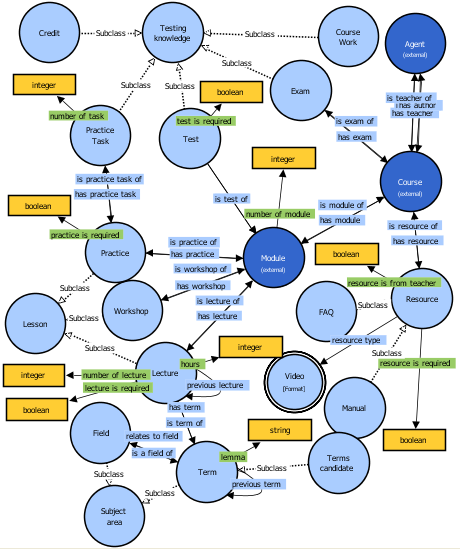
\includegraphics [scale=0.95] {ontology_edu}
  \caption{Основные классы и свойства онтологии учебных материалов.} 
  \label{img:ontology_edu}  
\end{figure}

\clearpage

 \section{Пример связывания объектов онтологии учебных материалов}\label{APP_A_EXMPL}

\begin{figure} [h] 
  \center
  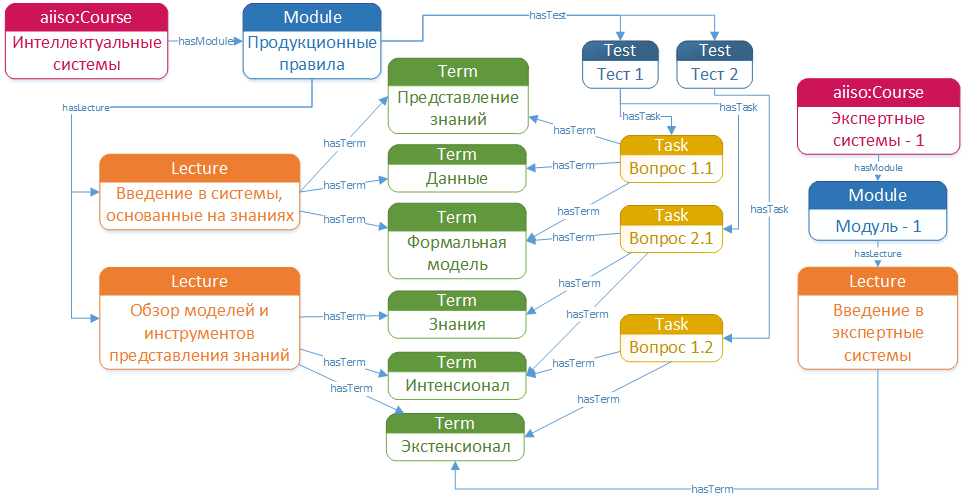
\includegraphics [scale=0.65] {ontology_edu_example_full}
  \caption{Пример связывания объектов онтологии учебных материалов.} 
  \label{img:ontology_edu_example_full}  
\end{figure}

\clearpage

 \section{Онтологическая модель тестов}\label{APP_A_TEST}

\begin{figure} [h] 
  \center
  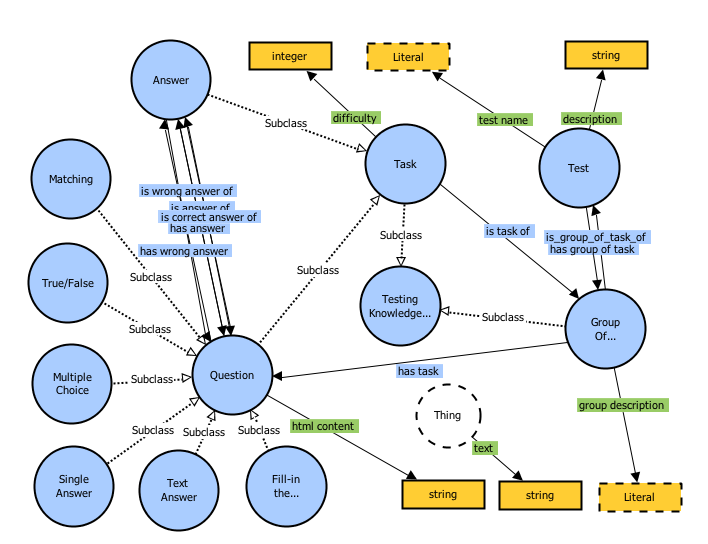
\includegraphics [scale=0.65] {ontology_test}
  \caption{Основные классы и свойства онтологии тестов.} 
  \label{img:ontology_test}  
\end{figure}

\clearpage

 \section{Онтологическая модель действий студента в системе электронного обучения}\label{APP_A_ACTION}

\begin{figure} [h] 
  \center
  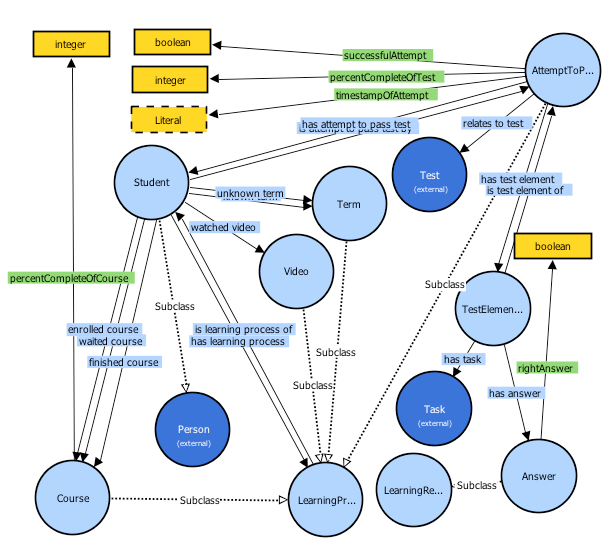
\includegraphics [scale=0.75] {ontology_action}
  \caption{Основные классы и свойства онтологии действий студента в системе электронного обучения.} 
  \label{img:ontology_action}  
\end{figure}

\clearpage

 \section{Онтологическая модель оценки знаний студентов}\label{APP_A_KNOW}

\begin{figure} [h] 
  \center
  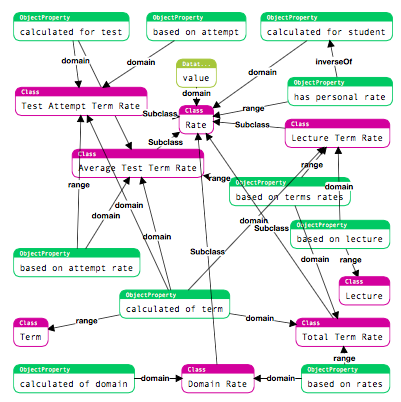
\includegraphics [scale=1.1] {ontology_know}
  \caption{Основные классы и оценки знаний студентов.} 
  \label{img:ontology_know}  
\end{figure}

\clearpage

\chapter{Отображение данных в формате XML в семантический формат} \label{APP_B_XML_MAP}


\begin{table}[h!]
\centering
\caption{Результаты преобразования на основе отображения учебного теста в формате XML в семантический формат}
\label{table:1}

\begin{tabular}{ |c|  }
  \hline
 \textbf{Исходные данные в XML коде}
 \\
 \hline
 \begin{lstlisting}
<test module="m_InterferenceAndCoherence" 
    module_ns="Phisics"
    uri="TestOfInterferenceAndDiffractionFrenel" 
    name="Test Of Interference And Diffraction Frenel">
</test>
 \end{lstlisting}
 \\
 \hline
  \textbf{Код отображения}
  \\
  \hline
\begin{lstlisting}
<rule id="test" nodeBase="//test" 
    owlType="learningRu:Test" 
    instanceNamespace="openeduTests"
    objectId="{./@uri}" 
    objectLabel="{./@name}">
    <objectPropertyMapping nodeBase="." 
        instanceNamespace="openeduTests"
        value="{./@name}" 
        owlProperty="ifmotest:hasGroupOfTasks" 
        referredRule="task_group" />
</rule>
\end{lstlisting}
    \\
 \hline
\textbf{Результат в RDF/XML коде}
\\
  \hline
  \begin{lstlisting}
<rdf:Description 
    rdf:about="http://openedu.ifmo.ru/tests/
    TestOfInterferenceAndDiffractionFrenel">
  <rdf:type 
    rdf:resource="http://www.semanticweb.org/
    k0shk/ontologies/2013/5/learning#Test"/>
  <label xmlns="http://www.w3.org/2000/01/rdf-schema#">
    Test Of Interference And Diffraction Frenel
  </label>
  <hasGroupOfTasks 
    xmlns="http://www.semanticweb.org/
    fedulity/ontologies/2014/4/untitled-ontology-13#" 
    rdf:resource="http://openedu.ifmo.ru/tests/
    Test_Of_Interference_And_Diffraction_Frenel"/>
</rdf:Description>
\end{lstlisting}

\\
 \hline
\end{tabular}

\end{table}

\clearpage


\chapter{Интерфейсы аналитических страниц учебных материалов} \label{APP_C}

 \section{Содержание электронного курса}\label{APP_C_COURSE_FIELD}


\begin{figure} [h] 
  \center
  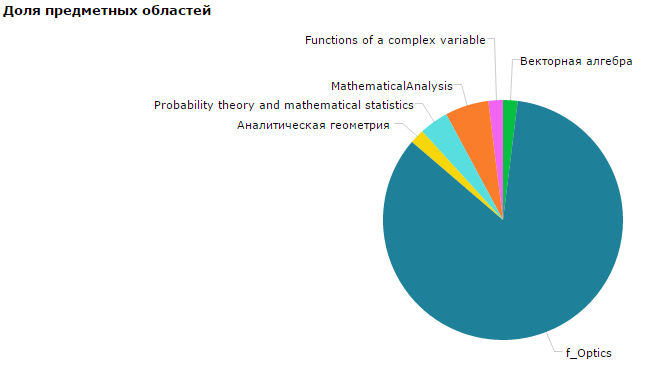
\includegraphics [width=\textwidth] {anl_screen_course_field}
\caption{Интерфейс анализа долей предметных областей в содержании курса.}
  \label{img:anl_screen_course_field}  
\end{figure}

\clearpage

 \section{Покрытие лекций тестами в контексте учебного модуля}\label{APP_C_COVER}


\begin{figure} [h] 
  \center
  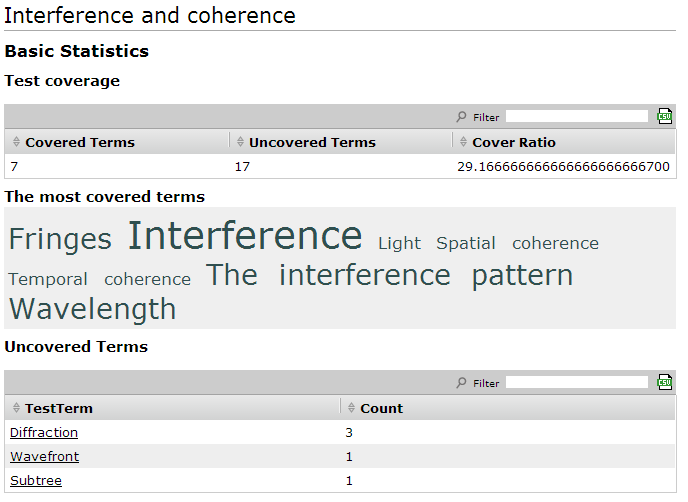
\includegraphics [width=\textwidth] {anl_screen_cover}
\caption{Интерфейс статистики покрытия модуля тестами в аналитической странице модуля.}
  \label{img:anl_screen_cover}  
\end{figure}

\begin{figure} [h] 
  \center
  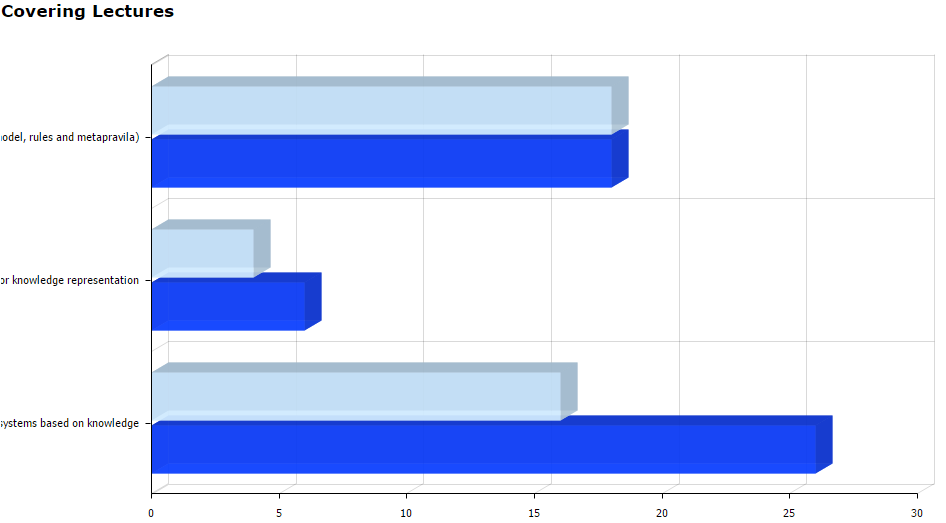
\includegraphics [width=\textwidth] {anl_screen_cover_lect}
\caption{Интерфейс статистики покрытия лекций тестами в аналитической странице модуля.}
  \label{img:anl_screen_cover_lect}  
\end{figure}

\clearpage


 \section{Проблемные концепты в контексте учебного модуля}\label{APP_C_PROBLEM}


\begin{figure} [h] 
  \center
  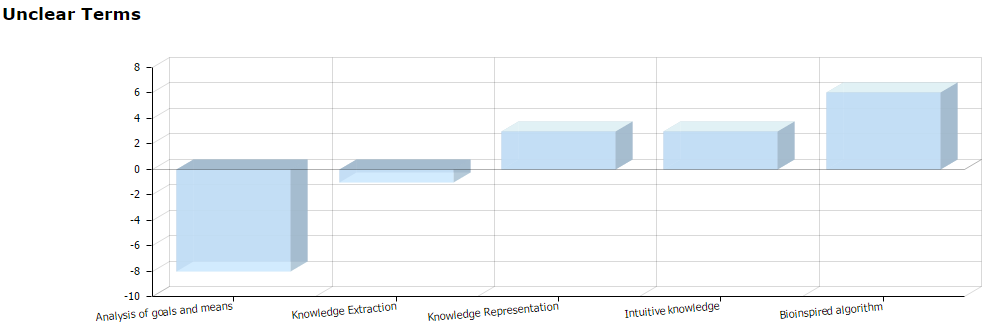
\includegraphics [width=\textwidth] {anl_screen_problem}
\caption{Интерфейс рейтинга проблемных концептов в аналитической странице модуля.}
  \label{img:anl_screen_problem}  
\end{figure}

\clearpage


\chapter{Интерфейсы системы электронного обучения ECOLE} \label{APP_D}

 \section{Интерфейс учебных материалов}\label{APP_D_STUD_EDU}

\begin{figure} [h] 
  \center
  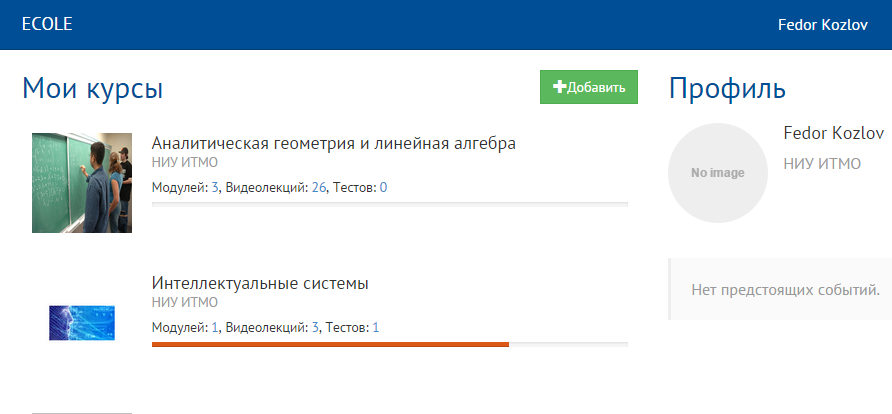
\includegraphics [width=\textwidth] {user_screen_init}
  \caption {Интерфейс списка курсов в системе ECOLE} 
  \label{fig:user_screen_init}
\end{figure}

\begin{figure} [h] 
  \center
  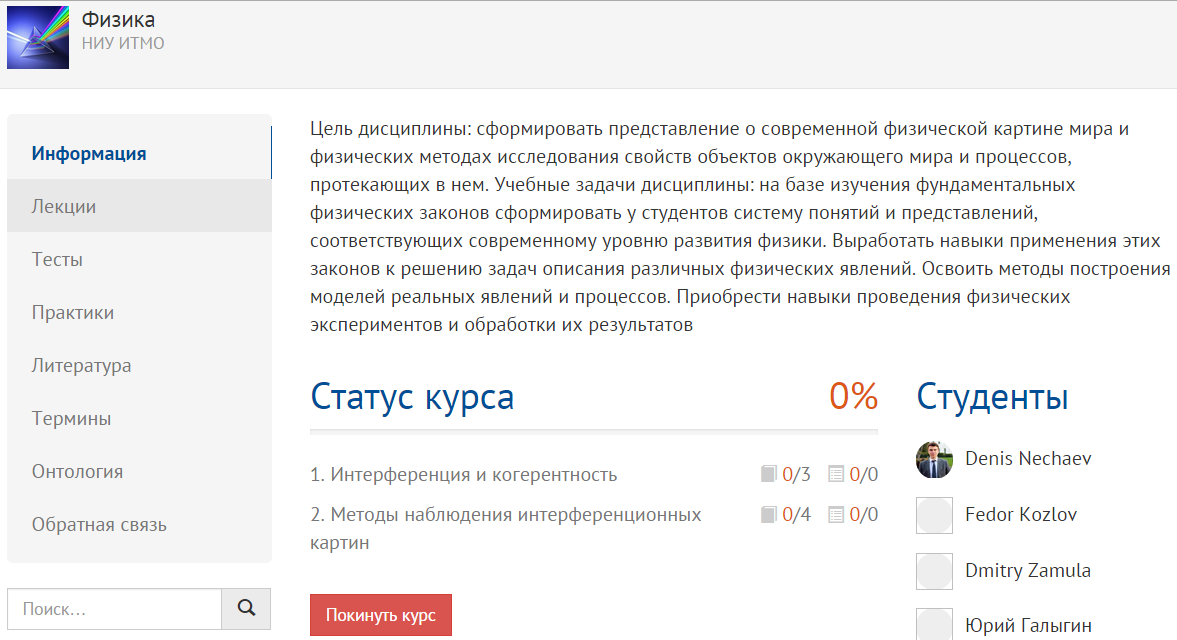
\includegraphics [width=\textwidth] {user_screen_course}
  \caption {Интерфейс курса в системе ECOLE} 
  \label{fig:user_screen_course}
\end{figure}

\begin{figure} [h] 
  \center
  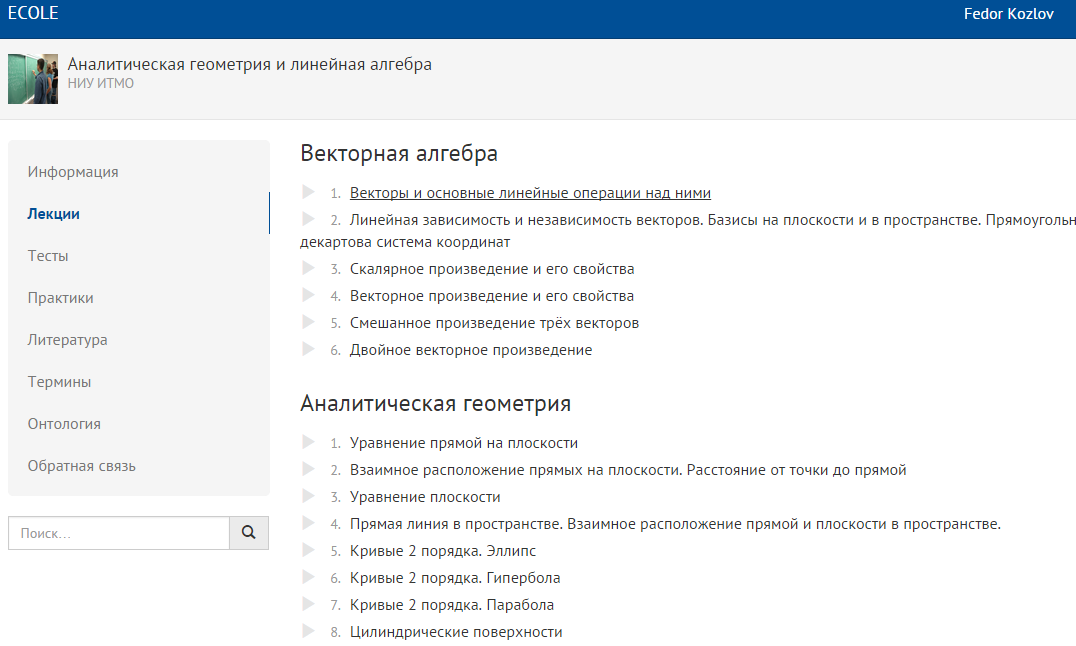
\includegraphics [width=\textwidth] {user_screen_lect_all}
  \caption {Интерфейс списка лекций в системе ECOLE} 
  \label{fig:user_screen_lect_all}
\end{figure}

\begin{figure} [h] 
  \center
  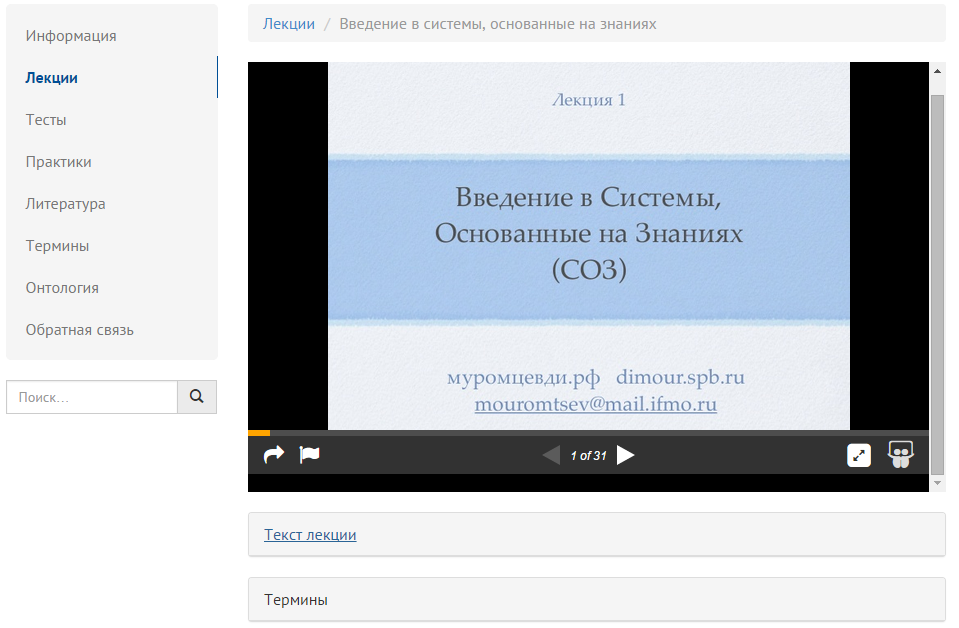
\includegraphics [width=\textwidth] {user_screen_lect}
  \caption {Интерфейс лекции в системе ECOLE} 
  \label{fig:user_screen_lect}
\end{figure}

\begin{figure} [h] 
  \center
  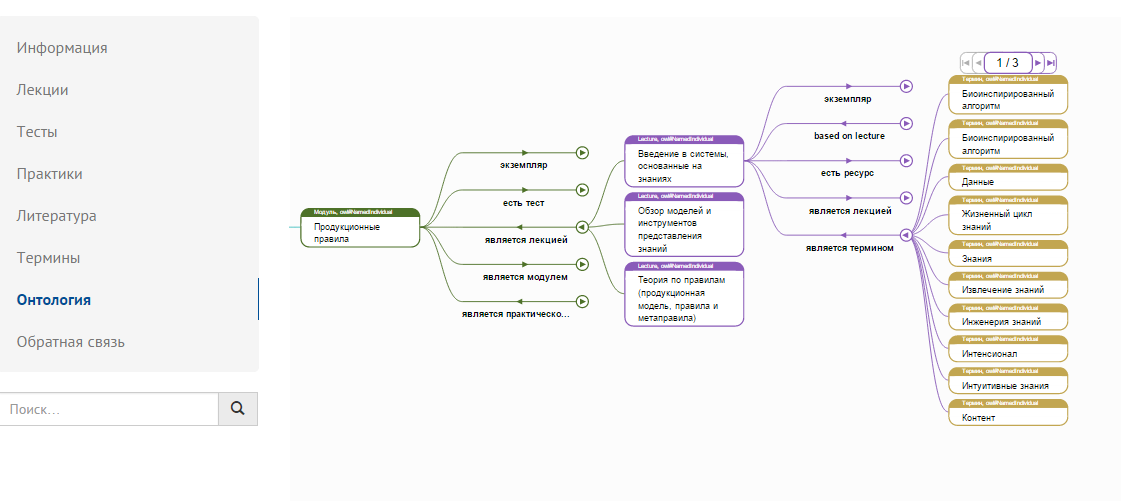
\includegraphics [width=\textwidth] {user_screen_graph}
  \caption {Интерфейс представления учебных материалов в виде интерактивного графа в системе ECOLE} 
  \label{fig:user_screen_graph}
\end{figure}

\clearpage


 \section{Интерфейс тестов}\label{APP_D_STUD_TEST}

\begin{figure} [h] 
  \center
  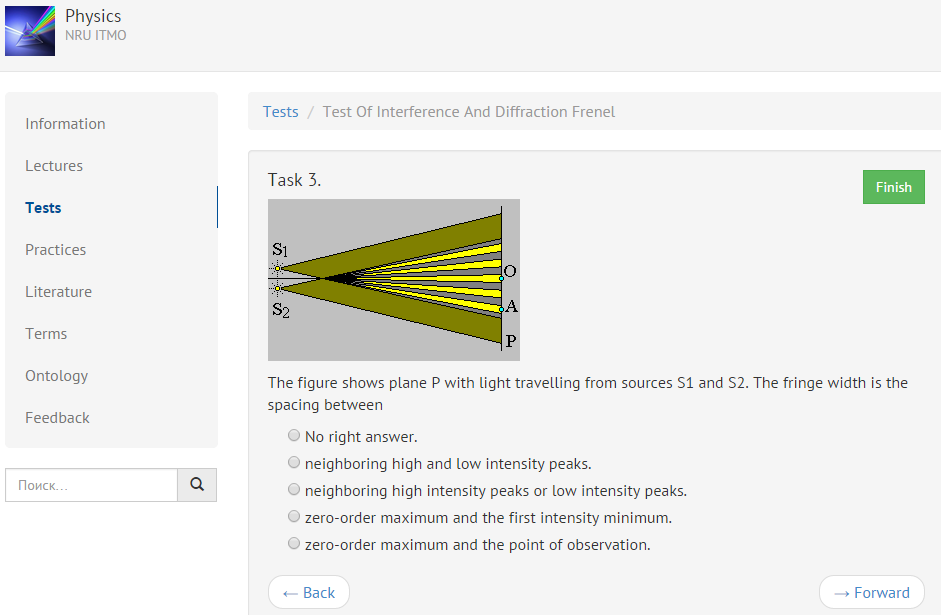
\includegraphics [width=\textwidth] {user_screen_test}
  \caption {Интерфейс ответов на задания тестов в системе ECOLE} 
  \label{fig:user_screen_test}
\end{figure}

\begin{figure} [h] 
  \center
  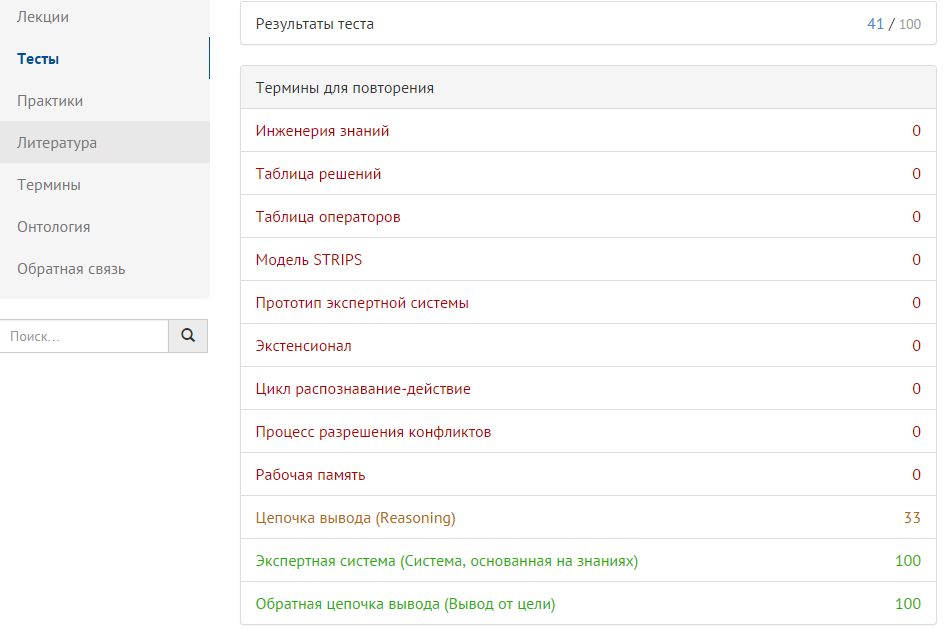
\includegraphics [width=\textwidth] {user_screen_test_result}
  \caption {Интерфейс результатов прохождения теста в системе ECOLE} 
  \label{fig:user_screen_test_result}
\end{figure}


\clearpage

 \section{Интерфейс оценки знаний студентом концептов и предметных областей }\label{APP_D_STUD_KNOW_TOTAL}

\begin{figure} [h] 
  \center
  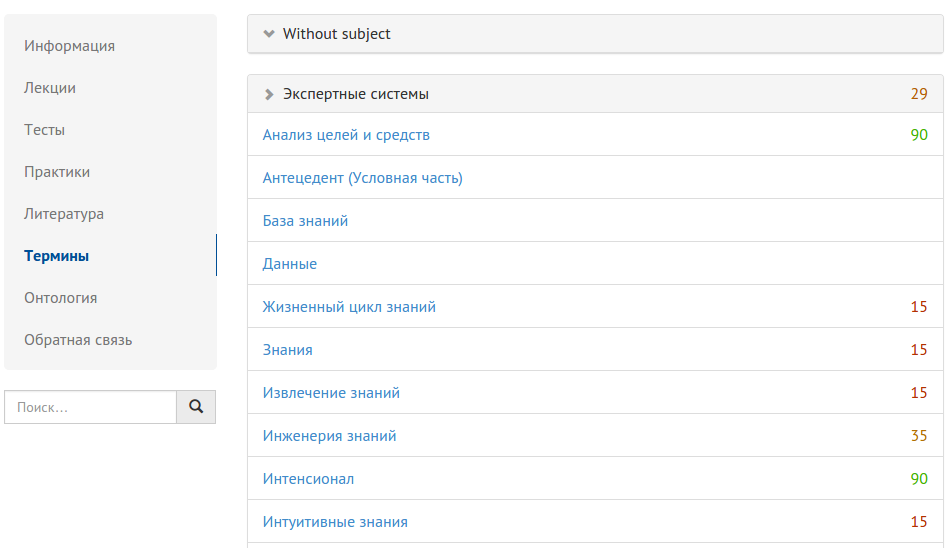
\includegraphics [width=\textwidth] {user_screen_result}
  \caption {Интерфейс списка предметных областей и терминов с рейтингами знаний в системе ECOLE} 
  \label{fig:user_screen_result}
\end{figure}

\clearpage


\chapter{Результаты эксперимента по анализу электронного курса <<Интеллектуальные системы>> в системе ECOLE} \label{APP_E}

 \section{Анализ объема и покрытия тестами лекций}\label{APP_E_COVER}

\begin{figure} [h] 
  \center
  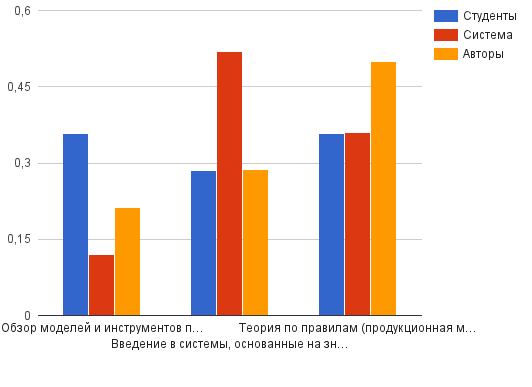
\includegraphics [width=\textwidth] {exp_lect_scale}
  \caption {Сравнительная диаграмма оценки объема лекций в электронном курсе}
  \label{fig:exp_lect_scale}
\end{figure}


\begin{figure} [h] 
  \center
  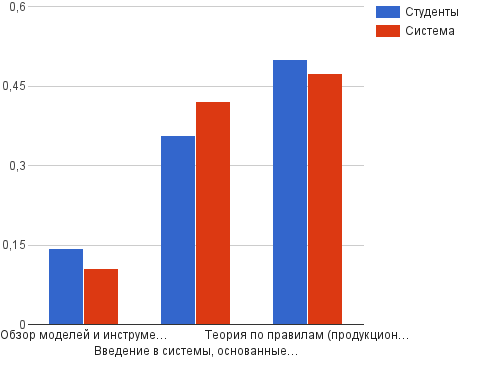
\includegraphics [width=\textwidth] {exp_lect_cover}
  \caption {Сравнительная диаграмма оценки покрытия лекций тестами в электронном курсе}
  \label{fig:exp_lect_cover}
\end{figure}



\clearpage


 \section{Анализ проблемных концептов электронного курса}\label{APP_E_PROBLEM}

\begin{figure} [h] 
  \center
  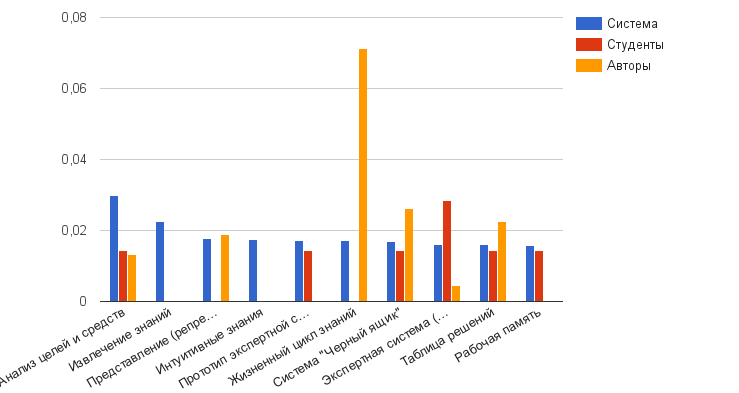
\includegraphics [width=\textwidth] {exp_problem_superfull}
  \caption {Сравнительная диаграмма оценки проблемных концептов в электронном курсе}
  \label{fig:exp_problem_superfull}
\end{figure}


\clearpage

 \section{Анализ значимости концептов электронного курса}\label{APP_E_IMPORT}


\begin{figure} [h] 
  \center
  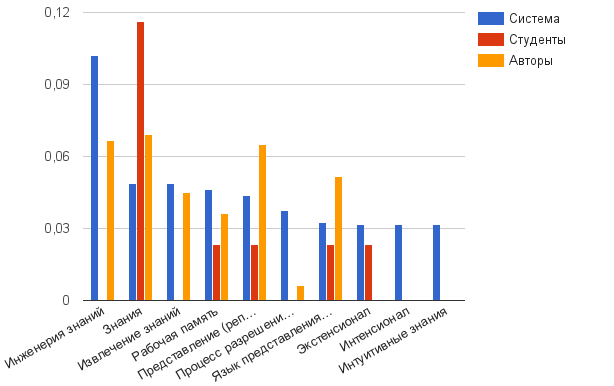
\includegraphics [width=\textwidth] {exp_problem_full}
  \caption {Сравнительная диаграмма оценки значимости концептов в электронном курсе}
  \label{fig:exp_problem_full}
\end{figure}

\begin{figure} [h] 
  \center
  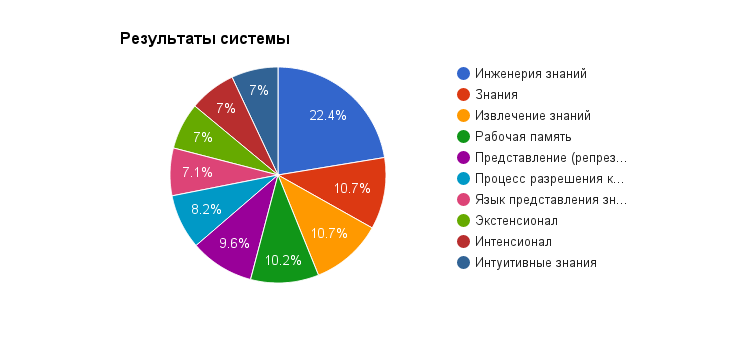
\includegraphics [width=\textwidth] {exp_problem_sys}
  \caption {Оценка значимости концептов системой в электронном курсе}
  \label{fig:exp_problem_sys}
\end{figure}

\begin{figure} [h] 
  \center
  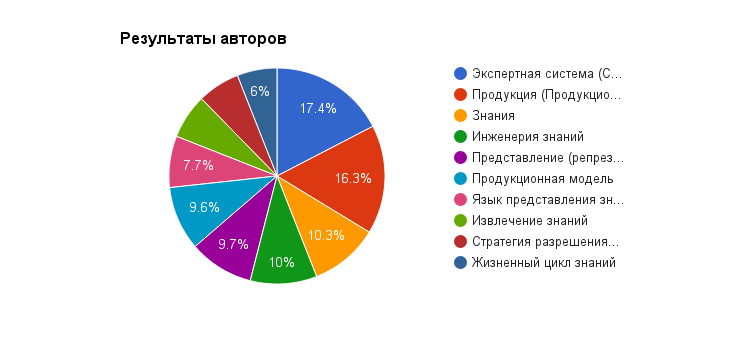
\includegraphics [width=\textwidth] {exp_problem_auth}
  \caption {Оценка значимости концептов авторами в электронном курсе}
  \label{fig:exp_problem_auth}
\end{figure}

\begin{figure} [h] 
  \center
  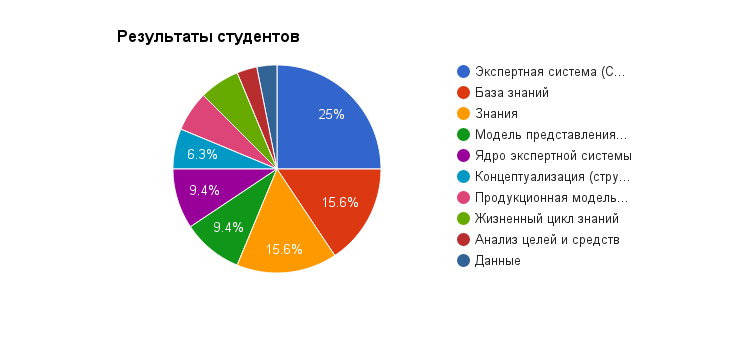
\includegraphics [width=\textwidth] {exp_problem_stud}
  \caption {Оценка значимости концептов студентами в электронном курсе}
  \label{fig:exp_problem_stud}
\end{figure}


\clearpage


 \section{Оценка знаний студентами предметной области электронного курса}\label{APP_E_RATE}

\begin{figure} [h] 
  \center
  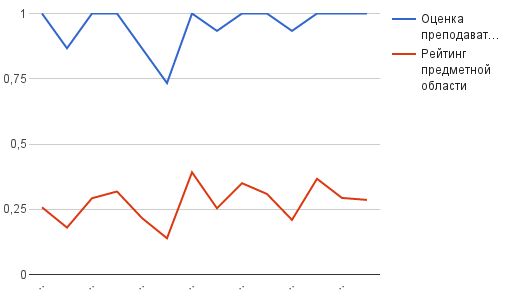
\includegraphics [width=\textwidth] {exp_stud_rate}
  \caption {Сравнительная диаграмма оценки знаний студентами предметной области в электронном курсе}
  \label{fig:exp_stud_rate}
\end{figure}


\clearpage